\chapter{樹}

LeetCode 上二叉樹的節點定義如下:
\begin{Code}
// 樹的節點
struct TreeNode {
    int val;
    TreeNode *left;
    TreeNode *right;
    TreeNode(int x) : val(x), left(nullptr), right(nullptr) { }
};
\end{Code}


\section{二叉樹的遍歷} %%%%%%%%%%%%%%%%%%%%%%%%%%%%%%

樹的遍歷有兩類:深度優先遍歷和寬度優先遍歷。深度優先遍歷又可分為兩種:先根(次序)遍歷和後根(次序)遍歷。

樹的先根遍歷是:先訪問樹的根結點,然後依次先根遍歷根的各棵子樹。樹的先跟遍歷的結果與對應二叉樹(孩子兄弟表示法)的先序遍歷的結果相同。

樹的後根遍歷是:先依次後根遍歷樹根的各棵子樹,然後訪問根結點。樹的後跟遍歷的結果與對應二叉樹的中序遍歷的結果相同。

二叉樹的先根遍歷有:\textbf{先序遍歷}(root->left->right),root->right->left;後根遍歷有:\textbf{後序遍歷}(left->right->root),right->left->root;二叉樹還有個一般的樹沒有的遍歷次序,\textbf{中序遍歷}(left->root->right)。


\subsection{Binary Tree Preorder Traversal}
\label{sec:binary-tree-preorder-traversal}


\subsubsection{描述}
Given a binary tree, return the \emph{preorder} traversal of its nodes' values.

For example:
Given binary tree \code{\{1,\#,2,3\}},
\begin{Code}
 1
  \
   2
  /
 3
\end{Code}
return \code{\[1,2,3\]}.

Note: Recursive solution is trivial, could you do it iteratively?


\subsubsection{分析}
用棧或者Morris遍歷。


\subsubsection{棧}
\begin{Code}
// LeetCode, Binary Tree Preorder Traversal
// 使用棧,時間複雜度O(n),空間複雜度O(n)
class Solution {
public:
    vector<int> preorderTraversal(TreeNode *root) {
        vector<int> result;
        stack<const TreeNode *> s;
        if (root != nullptr) s.push(root);

        while (!s.empty()) {
            const TreeNode *p = s.top();
            s.pop();
            result.push_back(p->val);

            if (p->right != nullptr) s.push(p->right);
            if (p->left != nullptr) s.push(p->left);
        }
        return result;
    }
};
\end{Code}


\subsubsection{Morris先序遍歷}
\begin{Code}
// LeetCode, Binary Tree Preorder Traversal
// Morris先序遍歷,時間複雜度O(n),空間複雜度O(1)
class Solution {
public:
    vector<int> preorderTraversal(TreeNode *root) {
        vector<int> result;
        TreeNode *cur = root, *prev = nullptr;

        while (cur != nullptr) {
            if (cur->left == nullptr) {
                result.push_back(cur->val);
                prev = cur; /* cur剛剛被訪問過 */
                cur = cur->right;
            } else {
                /* 查找前驅 */
                TreeNode *node = cur->left;
                while (node->right != nullptr && node->right != cur)
                    node = node->right;

                if (node->right == nullptr) { /* 還沒線索化,則建立線索 */
                    result.push_back(cur->val); /* 僅這一行的位置與中序不同 */
                    node->right = cur;
                    prev = cur; /* cur剛剛被訪問過 */
                    cur = cur->left;
                } else {    /* 已經線索化,則刪除線索  */
                    node->right = nullptr;
                    /* prev = cur; 不能有這句,cur已經被訪問 */
                    cur = cur->right;
                }
            }
        }
        return result;
    }
};
\end{Code}


\subsubsection{相關題目}
\begindot
\item Binary Tree Inorder Traversal,見 \S \ref{sec:binary-tree-inorder-traversal}
\item Binary Tree Postorder Traversal,見 \S \ref{sec:binary-tree-postorder-traversal}
\item Recover Binary Search Tree,見 \S \ref{sec:recover-binary-search-tree}
\myenddot


\subsection{Binary Tree Inorder Traversal}
\label{sec:binary-tree-inorder-traversal}


\subsubsection{描述}
Given a binary tree, return the \emph{inorder} traversal of its nodes' values.

For example:
Given binary tree \code{\{1,\#,2,3\}},
\begin{Code}
 1
  \
   2
  /
 3
\end{Code}
return \code{\[1,3,2\]}.

Note: Recursive solution is trivial, could you do it iteratively?


\subsubsection{分析}
用棧或者Morris遍歷。


\subsubsection{棧}
\begin{Code}
// LeetCode, Binary Tree Inorder Traversal
// 使用棧,時間複雜度O(n),空間複雜度O(n)
class Solution {
public:
    vector<int> inorderTraversal(TreeNode *root) {
        vector<int> result;
        stack<const TreeNode *> s;
        const TreeNode *p = root;

        while (!s.empty() || p != nullptr) {
            if (p != nullptr) {
                s.push(p);
                p = p->left;
            } else {
                p = s.top();
                s.pop();
                result.push_back(p->val);
                p = p->right;
            }
        }
        return result;
    }
};
\end{Code}


\subsubsection{Morris中序遍歷}
\begin{Code}
// LeetCode, Binary Tree Inorder Traversal
// Morris中序遍歷,時間複雜度O(n),空間複雜度O(1)
class Solution {
public:
    vector<int> inorderTraversal(TreeNode *root) {
        vector<int> result;
        TreeNode *cur = root, *prev = nullptr;

        while (cur != nullptr) {
            if (cur->left == nullptr) {
                result.push_back(cur->val);
                prev = cur;
                cur = cur->right;
            } else {
                /* 查找前驅 */
                TreeNode *node = cur->left;
                while (node->right != nullptr && node->right != cur)
                    node = node->right;

                if (node->right == nullptr) { /* 還沒線索化,則建立線索 */
                    node->right = cur;
                    /* prev = cur; 不能有這句,cur還沒有被訪問 */
                    cur = cur->left;
                } else {    /* 已經線索化,則訪問節點,並刪除線索  */
                    result.push_back(cur->val);
                    node->right = nullptr;
                    prev = cur;
                    cur = cur->right;
                }
            }
        }
        return result;
    }
};
\end{Code}


\subsubsection{相關題目}
\begindot
\item Binary Tree Preorder Traversal,見 \S \ref{sec:binary-tree-preorder-traversal}
\item Binary Tree Postorder Traversal,見 \S \ref{sec:binary-tree-postorder-traversal}
\item Recover Binary Search Tree,見 \S \ref{sec:recover-binary-search-tree}
\myenddot


\subsection{Binary Tree Postorder Traversal}
\label{sec:binary-tree-postorder-traversal}


\subsubsection{描述}
Given a binary tree, return the \emph{postorder} traversal of its nodes' values.

For example:
Given binary tree \code{\{1,\#,2,3\}},
\begin{Code}
 1
  \
   2
  /
 3
\end{Code}
return \code{\[3,2,1\]}.

Note: Recursive solution is trivial, could you do it iteratively?


\subsubsection{分析}
用棧或者Morris遍歷。


\subsubsection{棧}
\begin{Code}
// LeetCode, Binary Tree Postorder Traversal
// 使用棧,時間複雜度O(n),空間複雜度O(n)
class Solution {
public:
    vector<int> postorderTraversal(TreeNode *root) {
        vector<int> result;
        stack<const TreeNode *> s;
        /* p,正在訪問的結點,q,剛剛訪問過的結點*/
        const TreeNode *p = root, *q = nullptr;

        do {
            while (p != nullptr) { /* 往左下走*/
                s.push(p);
                p = p->left;
            }
            q = nullptr;
            while (!s.empty()) {
                p = s.top();
                s.pop();
                /* 右孩子不存在或已被訪問,訪問之*/
                if (p->right == q) {
                    result.push_back(p->val);
                    q = p; /* 保存剛訪問過的結點*/
                } else {
                    /* 當前結點不能訪問,需第二次進棧*/
                    s.push(p);
                    /* 先處理右子樹*/
                    p = p->right;
                    break;
                }
            }
        } while (!s.empty());

        return result;
    }
};
\end{Code}


\subsubsection{Morris後序遍歷}
\begin{Code}
// LeetCode, Binary Tree Postorder Traversal
// Morris後序遍歷,時間複雜度O(n),空間複雜度O(1)
class Solution {
public:
    vector<int> postorderTraversal(TreeNode *root) {
        vector<int> result;
        TreeNode dummy(-1);
        TreeNode *cur, *prev = nullptr;
        std::function < void(const TreeNode*)> visit = 
            [&result](const TreeNode *node){
            result.push_back(node->val); 
        };

        dummy.left = root;
        cur = &dummy;
        while (cur != nullptr) {
            if (cur->left == nullptr) {
                prev = cur; /* 必須要有 */
                cur = cur->right;
            } else {
                TreeNode *node = cur->left;
                while (node->right != nullptr && node->right != cur)
                    node = node->right;

                if (node->right == nullptr) { /* 還沒線索化,則建立線索 */
                    node->right = cur;
                    prev = cur; /* 必須要有 */
                    cur = cur->left;
                } else { /* 已經線索化,則訪問節點,並刪除線索  */
                    visit_reverse(cur->left, prev, visit);
                    prev->right = nullptr;
                    prev = cur; /* 必須要有 */
                    cur = cur->right;
                }
            }
        }
        return result;
    }
private:
    // 逆轉路徑
    static void reverse(TreeNode *from, TreeNode *to) {
        TreeNode *x = from, *y = from->right, *z;
        if (from == to) return;

        while (x != to) {
            z = y->right;
            y->right = x;
            x = y;
            y = z;
        }
    }

    // 訪問逆轉後的路徑上的所有結點
    static void visit_reverse(TreeNode* from, TreeNode *to, 
                     std::function< void(const TreeNode*) >& visit) {
        TreeNode *p = to;
        reverse(from, to);

        while (true) {
            visit(p);
            if (p == from)
                break;
            p = p->right;
        }

        reverse(to, from);
    }
};
\end{Code}


\subsubsection{相關題目}
\begindot
\item Binary Tree Preorder Traversal,見 \S \ref{sec:binary-tree-preorder-traversal}
\item Binary Tree Inorder Traversal,見 \S \ref{sec:binary-tree-inorder-traversal}
\item Recover Binary Search Tree,見 \S \ref{sec:recover-binary-search-tree}
\myenddot


\subsection{Binary Tree Level Order Traversal}
\label{sec:binary-tree-level-order-traversal}


\subsubsection{描述}
Given a binary tree, return the level order traversal of its nodes' values. (ie, from left to right, level by level).

For example:
Given binary tree \code{\{3,9,20,\#,\#,15,7\}},
\begin{Code}
    3
   / \
  9  20
    /  \
   15   7
\end{Code}
return its level order traversal as:
\begin{Code}
[
  [3],
  [9,20],
  [15,7]
]
\end{Code}


\subsubsection{分析}
無


\subsubsection{遞歸版}
\begin{Code}
// LeetCode, Binary Tree Level Order Traversal
// 遞歸版,時間複雜度O(n),空間複雜度O(n)
class Solution {
public:
    vector<vector<int> > levelOrder(TreeNode *root) {
        vector<vector<int>> result;
        traverse(root, 1, result);
        return result;
    }

    void traverse(TreeNode *root, size_t level, vector<vector<int>> &result) {
        if (!root) return;

        if (level > result.size())
            result.push_back(vector<int>());

        result[level-1].push_back(root->val);
        traverse(root->left, level+1, result);
        traverse(root->right, level+1, result);
    }
};
\end{Code}


\subsubsection{迭代版}
\begin{Code}
// LeetCode, Binary Tree Level Order Traversal
// 迭代版,時間複雜度O(n),空間複雜度O(1)
class Solution {
public:
    vector<vector<int> > levelOrder(TreeNode *root) {
        vector<vector<int> > result;
        queue<TreeNode*> current, next;
        
        if(root == nullptr) {
            return result;
        } else {
            current.push(root);
        }

        while (!current.empty()) {
            vector<int> level; // elments in one level
            while (!current.empty()) {
                TreeNode* node = current.front();
                current.pop();
                level.push_back(node->val);
                if (node->left != nullptr) next.push(node->left);
                if (node->right != nullptr) next.push(node->right);
            }
            result.push_back(level);
            swap(next, current);
        }
        return result;
    }
};
\end{Code}


\subsubsection{相關題目}
\begindot
\item Binary Tree Level Order Traversal II,見 \S \ref{sec:binary-tree-level-order-traversal-ii}
\item Binary Tree Zigzag Level Order Traversal,見 \S \ref{sec:binary-tree-zigzag-level-order-traversal}
\myenddot


\subsection{Binary Tree Level Order Traversal II}
\label{sec:binary-tree-level-order-traversal-ii}


\subsubsection{描述}
Given a binary tree, return the bottom-up level order traversal of its nodes' values. (ie, from left to right, level by level from leaf to root).

For example:
Given binary tree \code{\{3,9,20,\#,\#,15,7\}},
\begin{Code}
    3
   / \
  9  20
    /  \
   15   7
\end{Code}
return its bottom-up level order traversal as:
\begin{Code}
[
  [15,7]
  [9,20],
  [3],
]
\end{Code}


\subsubsection{分析}
在上一題(見\S \ref{sec:binary-tree-level-order-traversal})的基礎上,\fn{reverse()}一下即可。


\subsubsection{遞歸版}
\begin{Code}
// LeetCode, Binary Tree Level Order Traversal II
// 遞歸版,時間複雜度O(n),空間複雜度O(n)
class Solution {
public:
    vector<vector<int> > levelOrderBottom(TreeNode *root) {
        vector<vector<int>> result;
        traverse(root, 1, result);
        std::reverse(result.begin(), result.end()); // 比上一題多此一行
        return result;
    }

    void traverse(TreeNode *root, size_t level, vector<vector<int>> &result) {
        if (!root) return;

        if (level > result.size())
            result.push_back(vector<int>());

        result[level-1].push_back(root->val);
        traverse(root->left, level+1, result);
        traverse(root->right, level+1, result);
    }
};
\end{Code}


\subsubsection{迭代版}
\begin{Code}
// LeetCode, Binary Tree Level Order Traversal II
// 迭代版,時間複雜度O(n),空間複雜度O(1)
class Solution {
public:
    vector<vector<int> > levelOrderBottom(TreeNode *root) {
        vector<vector<int> > result;
        if(root == nullptr) return result;

        queue<TreeNode*> current, next;
        vector<int> level; // elments in level level

        current.push(root);
        while (!current.empty()) {
            while (!current.empty()) {
                TreeNode* node = current.front();
                current.pop();
                level.push_back(node->val);
                if (node->left != nullptr) next.push(node->left);
                if (node->right != nullptr) next.push(node->right);
            }
            result.push_back(level);
            level.clear();
            swap(next, current);
        }
        reverse(result.begin(), result.end()); // 比上一題多此一行
        return result;
    }
};
\end{Code}


\subsubsection{相關題目}
\begindot
\item Binary Tree Level Order Traversal,見 \S \ref{sec:binary-tree-level-order-traversal}
\item Binary Tree Zigzag Level Order Traversal,見 \S \ref{sec:binary-tree-zigzag-level-order-traversal}
\myenddot


\subsection{Binary Tree Zigzag Level Order Traversal}
\label{sec:binary-tree-zigzag-level-order-traversal}


\subsubsection{描述}
Given a binary tree, return the zigzag level order traversal of its nodes' values. (ie, from left to right, then right to left for the next level and alternate between).

For example:
Given binary tree \code{{3,9,20,\#,\#,15,7}},
\begin{Code}
    3
   / \
  9  20
    /  \
   15   7
\end{Code}
return its zigzag level order traversal as:
\begin{Code}
[
  [3],
  [20,9],
  [15,7]
]
\end{Code}


\subsubsection{分析}
廣度優先遍歷,用一個bool記錄是從左到右還是從右到左,每一層結束就翻轉一下。


\subsubsection{遞歸版}
\begin{Code}
// LeetCode, Binary Tree Zigzag Level Order Traversal
// 遞歸版,時間複雜度O(n),空間複雜度O(n)
class Solution {
public:
    vector<vector<int> > zigzagLevelOrder(TreeNode *root) {
        vector<vector<int>> result;
        traverse(root, 1, result, true);
        return result;
    }

    void traverse(TreeNode *root, size_t level, vector<vector<int>> &result,
            bool left_to_right) {
        if (!root) return;

        if (level > result.size())
            result.push_back(vector<int>());

        if (left_to_right)
            result[level-1].push_back(root->val);
        else
            result[level-1].insert(result[level-1].begin(), root->val);

        traverse(root->left, level+1, result, !left_to_right);
        traverse(root->right, level+1, result, !left_to_right);
    }
};
\end{Code}

\subsubsection{迭代版}
\begin{Code}
// LeetCode, Binary Tree Zigzag Level Order Traversal
// 廣度優先遍歷,用一個bool記錄是從左到右還是從右到左,每一層結束就翻轉一下。
// 迭代版,時間複雜度O(n),空間複雜度O(n)
class Solution {
public:
    vector<vector<int> > zigzagLevelOrder(TreeNode *root) {
        vector<vector<int> > result;
        queue<TreeNode*> current, next;
        bool left_to_right = true;
        
        if(root == nullptr) {
            return result;
        } else {
            current.push(root);
        }

        while (!current.empty()) {
            vector<int> level; // elments in one level
            while (!current.empty()) {
                TreeNode* node = current.front();
                current.pop();
                level.push_back(node->val);
                if (node->left != nullptr) next.push(node->left);
                if (node->right != nullptr) next.push(node->right);
            }
            if (!left_to_right) reverse(level.begin(), level.end());
            result.push_back(level);
            left_to_right = !left_to_right;
            swap(next, current);
        }
        return result;
    }
};
\end{Code}


\subsubsection{相關題目}
\begindot
\item Binary Tree Level Order Traversal,見 \S \ref{sec:binary-tree-level-order-traversal}
\item Binary Tree Level Order Traversal II,見 \S \ref{sec:binary-tree-level-order-traversal-ii}
\myenddot

\subsection{Binary Tree Right side View}
\label{sec:binary-tree-right-side-view}


\subsubsection{描述}
Given a binary tree, imagine yourself standing on the right side of it, return the values of the nodes you can see ordered from top to bottom.

For example:
Given binary tree \code{{3,9,20,\#,\#,15,7}},
\begin{Code}
    3     <--
   / \
  9  20   <--
    /  \
   15   7 <--
\end{Code}
return as:
\begin{Code}
[3,20,7]
\end{Code}


\subsubsection{分析}
雙 queue BFS zigzag travel, 只選最右

\subsubsection{遞歸版}
\begin{Code}
// LeetCode, Binary Tree Zigzag Level Order Traversal
// 遞歸版,時間複雜度O(n),空間複雜度O(n)
class Solution {
public:
    vector<int> rightSideView(TreeNode* root) {
        if (root == nullptr) return vector<int>();
        vector<int> result;
        
        // 雙 queue BFS zigzag travel
        queue<TreeNode*> cur, next;
        cur.push(root);
        while (!cur.empty())
        {
            while (!cur.empty())
            {
                TreeNode *p = cur.front();
                cur.pop();
                
                if (cur.size() == 0) // 只選最右
                    result.push_back(p->val);
                
                if (p->left) next.push(p->left);
                if (p->right) next.push(p->right);
            }
            swap(cur, next);
        }
        
        return result;
    }
};
\end{Code}


\subsubsection{相關題目}
\begindot
\item Binary Tree Level Order Traversal,見 \S \ref{sec:binary-tree-level-order-traversal}
\item Binary Tree Level Order Traversal II,見 \S \ref{sec:binary-tree-level-order-traversal-ii}
\myenddot

\subsection{Recover Binary Search Tree}
\label{sec:recover-binary-search-tree}


\subsubsection{描述}
Two elements of a binary search tree (BST) are swapped by mistake.

Recover the tree without changing its structure.

Note: A solution using $O(n)$ space is pretty straight forward. Could you devise a constant space solution?


\subsubsection{分析}
$O(n)$空間的解法是,開一個指針數組,中序遍歷,將節點指針依次存放到數組裏,然後尋找兩處逆向的位置,先從前往後找第一個逆序的位置,然後從後往前找第二個逆序的位置,交換這兩個指針的值。

中序遍歷一般需要用到棧,空間也是$O(n)$的,如何才能不使用棧?Morris中序遍歷。


\subsubsection{代碼}

\begin{Code}
// LeetCode, Recover Binary Search Tree
// Morris中序遍歷,時間複雜度O(n),空間複雜度O(1)
class Solution {
public:
    void recoverTree(TreeNode* root) {
        pair<TreeNode*, TreeNode*> broken;
        TreeNode* prev = nullptr;
        TreeNode* cur = root;

        while (cur != nullptr) {
            if (cur->left == nullptr) {
                detect(broken, prev, cur);
                prev = cur;
                cur = cur->right;
            } else {
                auto node = cur->left;

                while (node->right != nullptr && node->right != cur)
                    node = node->right;

                if (node->right == nullptr) {
                    node->right = cur;
                    //prev = cur; 不能有這句!因為cur還沒有被訪問
                    cur = cur->left;
                } else {
                    detect(broken, prev, cur);
                    node->right = nullptr;
                    prev = cur;
                    cur = cur->right;
                }
            }
        }

        swap(broken.first->val, broken.second->val);
    }

    void detect(pair<TreeNode*, TreeNode*>& broken, TreeNode* prev,
            TreeNode* current) {
        if (prev != nullptr && prev->val > current->val) {
            if (broken.first == nullptr) {
                broken.first = prev;
            } //不能用else,例如 {0,1},會導致最後 swap時second為nullptr,
              //會 Runtime Error
            broken.second = current;
        }
    }
};
\end{Code}


\subsubsection{相關題目}
\begindot
\item Binary Tree Inorder Traversal,見 \S \ref{sec:binary-tree-inorder-traversal}
\myenddot


\subsection{Same Tree}
\label{sec:same-tree}


\subsubsection{描述}
Given two binary trees, write a function to check if they are equal or not.

Two binary trees are considered equal if they are structurally identical and the nodes have the same value.


\subsubsection{分析}
無


\subsubsection{遞歸版}
遞歸版
\begin{Code}
// LeetCode, Same Tree
// 遞歸版,時間複雜度O(n),空間複雜度O(logn)
class Solution {
public:
    bool isSameTree(TreeNode *p, TreeNode *q) {
        if (!p && !q) return true;   // 終止條件
        if (!p || !q) return false;  // 剪枝
        return p->val == q->val      // 三方合併
                && isSameTree(p->left, q->left)
                && isSameTree(p->right, q->right);
    }
};
\end{Code}


\subsubsection{迭代版}
\begin{Code}
// LeetCode, Same Tree
// 迭代版,時間複雜度O(n),空間複雜度O(logn)
class Solution {
public:
    bool isSameTree(TreeNode *p, TreeNode *q) {
        stack<TreeNode*> s;
        s.push(p);
        s.push(q);

        while(!s.empty()) {
            p = s.top(); s.pop();
            q = s.top(); s.pop();

            if (!p && !q) continue;
            if (!p || !q) return false;
            if (p->val != q->val) return false;

            s.push(p->left);
            s.push(q->left);

            s.push(p->right);
            s.push(q->right);
        }
        return true;
    }
};
\end{Code}


\subsubsection{相關題目}
\begindot
\item Symmetric Tree,見 \S \ref{sec:symmetric-tree}
\myenddot

\subsection{Count Univalue Subtrees}
\label{sec:count-univalue-subtrees}


\subsubsection{描述}
Given a binary tree, count the number of uni-value subtrees.

A Uni-value subtree means all nodes of the subtree have the same value.

Example:

\begin{Code}
Input:  root = [5,1,5,5,5,null,5]

              5
             / \
            1   5
           / \   \
          5   5   5

Output: 4
\end{Code}

\subsubsection{分析}
無

\subsubsection{Pass Parent Values}
\begin{Code}
// LeetCode
// 迭代版,時間複雜度O(n),空間複雜度O(1)
class Solution {
public:
    int countUnivalSubtrees(TreeNode* root) {
        if (root == nullptr) return 0;

        int count = 0;
        DFS(root, count, root->val - 1);

        return count;
    }
private:
    bool DFS(TreeNode *root, int& count, int parVal) {
        if (root == nullptr) return true;

        int leftCount, rightCount; leftCount = rightCount = 0;
        bool isLeftUni = DFS(root->left, leftCount, root->val);
        bool isRightUni = DFS(root->right, rightCount, root->val);

        count += leftCount + rightCount;

        if (!isLeftUni || !isRightUni) return false;

        count++;

        return root->val == parVal;
    }
};
\end{Code}

\subsubsection{遞歸版}
\begin{Code}
// LeetCode
// 迭代版,時間複雜度O(n),空間複雜度O(logn)
class Solution {
public:
    int countUnivalSubtrees(TreeNode* root) {
        if (root == nullptr) return 0;

        int uniCount = 0;
        bool uniTrue = false;
        countUnivalSubtrees(root, uniCount, uniTrue);

        return uniCount;
    }
private:
    void countUnivalSubtrees(TreeNode *root, int& uniCount, bool& uniTrue) {
        if (root == nullptr) {
            uniCount = 0;
            uniTrue = false;
        }
        else if (root->left == nullptr && root->right == nullptr) {
            uniCount = 1;
            uniTrue = true;
        }
        else {
            int uniLeft, uniRight; uniLeft = uniRight = 0;
            bool isUniLeft, isUniRight; isUniLeft = isUniRight = false;
            countUnivalSubtrees(root->left, uniLeft, isUniLeft);
            countUnivalSubtrees(root->right, uniRight, isUniRight);

            // 三方比較
            if (root->left && root->right
               && (root->val == root->left->val && isUniLeft)
               && (root->val == root->right->val && isUniRight)) {
                uniLeft++;
                uniTrue = true;
            }
            else if (root->left && root->right == nullptr
                     && root->val == root->left->val && isUniLeft)
            { uniLeft++; uniTrue = true; } // 左邊比較
            else if (root->left == nullptr && root->right
                     && root->val == root->right->val && isUniRight)
            { uniRight++; uniTrue = true; } // 右邊比較

            uniCount = uniLeft + uniRight;
        }
    }
};
\end{Code}


\subsubsection{相關題目}
\begindot
\item Same Tree,見 \S \ref{sec:same-tree}
\myenddot

\subsection{Lowest Common Ancestor of Binary Tree}
\label{sec:lowest-common-ancestor-of-binary-tree}


\subsubsection{描述}
Given a binary tree, find the lowest common ancestor (LCA) of two given nodes in the tree.

According to the definition of LCA on Wikipedia: “The lowest common ancestor is defined between two nodes p and q as the lowest node in T that has both p and q as descendants (where we allow a node to be a descendant of itself).”

Given the following binary tree:  root = [3,5,1,6,2,0,8,null,null,7,4]

\begin{center}
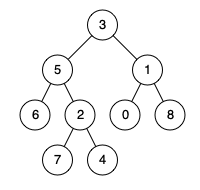
\includegraphics[width=100pt]{lowest-common-ancestor.png}\\
\figcaption{Loest common ancestor}\label{fig:lowest-common-ancestor}
\end{center}

Example 1:
\begin{Code}
Input: root = [3,5,1,6,2,0,8,null,null,7,4], p = 5, q = 1
Output: 3
Explanation: The LCA of nodes 5 and 1 is 3.
\end{Code}


Example 2:
\begin{Code}
Input: root = [3,5,1,6,2,0,8,null,null,7,4], p = 5, q = 4
Output: 5
Explanation: The LCA of nodes 5 and 4 is 5
, since a node can be a descendant of itself according to the LCA definition.
\end{Code}

\subsubsection{分析}
無


\subsubsection{遞歸版}
\begin{Code}
// LeetCode
// 遞歸版,時間複雜度O(n),空間複雜度O(1)
class Solution {
public:
    TreeNode* lowestCommonAncestor(TreeNode* root, TreeNode* p, TreeNode* q) {
        if (root == nullptr || p == nullptr || q == nullptr) return nullptr;
        if (root == p || root == q) return root;

        TreeNode *left = lowestCommonAncestor(root->left, p, q);
        TreeNode *right = lowestCommonAncestor(root->right, p, q);

        if (left && right)
            return root;
        else if (!left && !right)
            return nullptr;
        else if (!left)
            return right;
        else
            return left;
    }
};
\end{Code}


\subsubsection{相關題目}
\begindot
\item Same Tree,見 \S \ref{sec:same-tree}
\myenddot


\subsection{Symmetric Tree}
\label{sec:symmetric-tree}


\subsubsection{描述}
Given two binary trees, write a function to check if they are equal or not.

Two binary trees are considered equal if they are structurally identical and the nodes have the same value.


\subsubsection{分析}
無


\subsubsection{遞歸版}
\begin{Code}
// LeetCode, Symmetric Tree
// 遞歸版,時間複雜度O(n),空間複雜度O(logn)
class Solution {
public:
    bool isSymmetric(TreeNode *root) {
        if (root == nullptr) return true;
        return isSymmetric(root->left, root->right);
    }
    bool isSymmetric(TreeNode *p, TreeNode *q) {
        if (p == nullptr && q == nullptr) return true;   // 終止條件
        if (p == nullptr || q == nullptr) return false;  // 終止條件
        return p->val == q->val      // 三方合併
                && isSymmetric(p->left, q->right)
                && isSymmetric(p->right, q->left);
    }
};
\end{Code}


\subsubsection{迭代版}
\begin{Code}
// LeetCode, Symmetric Tree
// 迭代版,時間複雜度O(n),空間複雜度O(logn)
class Solution {
public:
    bool isSymmetric (TreeNode* root) {
        if (!root) return true;

        stack<TreeNode*> s;
        s.push(root->left);
        s.push(root->right);

        while (!s.empty ()) {
            auto p = s.top (); s.pop();
            auto q = s.top (); s.pop();

            if (!p && !q) continue;
            if (!p || !q) return false;
            if (p->val != q->val) return false;

            s.push(p->left);
            s.push(q->right);

            s.push(p->right);
            s.push(q->left);
        }

        return true;
    }
};
\end{Code}


\subsubsection{相關題目}
\begindot
\item Same Tree,見 \S \ref{sec:same-tree}
\myenddot


\subsection{Balanced Binary Tree}
\label{sec:balanced-binary-tree}


\subsubsection{描述}
Given a binary tree, determine if it is height-balanced.

For this problem, a height-balanced binary tree is defined as a binary tree in which the depth of the two subtrees of every node never differ by more than 1.


\subsubsection{分析}
無


\subsubsection{代碼}
\begin{Code}
// LeetCode, Balanced Binary Tree
// 時間複雜度O(n),空間複雜度O(logn)
class Solution {
public:
    bool isBalanced (TreeNode* root) {
        return balancedHeight (root) >= 0;
    }

    /**
     * Returns the height of `root` if `root` is a balanced tree,
     * otherwise, returns `-1`.
     */
    int balancedHeight (TreeNode* root) {
        if (root == nullptr) return 0;  // 終止條件

        int left = balancedHeight (root->left);
        int right = balancedHeight (root->right);

        if (left < 0 || right < 0 || abs(left - right) > 1) return -1;  // 剪枝

        return max(left, right) + 1; // 三方合併
    }
};
\end{Code}


\subsubsection{相關題目}
\begindot
\item 無
\myenddot


\subsection{Flatten Binary Tree to Linked List}
\label{sec:flatten-binary-tree-to-linked-list}


\subsubsection{描述}
Given a binary tree, flatten it to a linked list in-place.

For example, Given
\begin{Code}
         1
        / \
       2   5
      / \   \
     3   4   6
\end{Code}

The flattened tree should look like:
\begin{Code}
   1
    \
     2
      \
       3
        \
         4
          \
           5
            \
             6
\end{Code}

\subsubsection{分析}
無


\subsubsection{遞歸版1}
\begin{Code}
// LeetCode, Flatten Binary Tree to Linked List
// 遞歸版1,時間複雜度O(n),空間複雜度O(logn)
class Solution {
public:
    void flatten(TreeNode *root) {
        if (root == nullptr) return;  // 終止條件

        flatten(root->left);
        flatten(root->right);

        if (nullptr == root->left) return;

        // 三方合併,將左子樹所形成的鏈表插入到root和root->right之間
        TreeNode *p = root->left;
        while(p->right) p = p->right; //尋找左鏈表最後一個節點
        p->right = root->right;
        root->right = root->left;
        root->left = nullptr;
    }
};
\end{Code}


\subsubsection{遞歸版2}
\begin{Code}
// LeetCode, Flatten Binary Tree to Linked List
// 遞歸版2
// @author 王順達(http://weibo.com/u/1234984145)
// 時間複雜度O(n),空間複雜度O(logn)
class Solution {
public:
    void flatten(TreeNode *root) {
        flatten(root, NULL);
    }
private:
    // 把root所代表樹變成鏈表後,tail跟在該鏈表後面
    TreeNode *flatten(TreeNode *root, TreeNode *tail) {
        if (NULL == root) return tail;

        root->right = flatten(root->left, flatten(root->right, tail));
        root->left = NULL;
        return root;
    }
};
\end{Code}


\subsubsection{迭代版}
\begin{Code}
// LeetCode, Flatten Binary Tree to Linked List
// 迭代版,時間複雜度O(n),空間複雜度O(logn)
class Solution {
public:
    void flatten(TreeNode* root) {
        if (root == nullptr) return;

        stack<TreeNode*> s;
        s.push(root);

        while (!s.empty()) {
            auto p = s.top();
            s.pop();

            if (p->right)
                s.push(p->right);
            if (p->left)
                s.push(p->left);

            p->left = nullptr;
            if (!s.empty())
                p->right = s.top();
        }
    }
};
\end{Code}


\subsubsection{相關題目}
\begindot
\item 無
\myenddot


\subsection{Populating Next Right Pointers in Each Node II} %%%%%%%%%%%%%%%%%%%%%%%%%%%%%%
\label{sec:populating-next-right-pointers-in-each-node-ii}


\subsubsection{描述}
Follow up for problem "Populating Next Right Pointers in Each Node".

What if the given tree could be any binary tree? Would your previous solution still work?

Note: You may only use constant extra space.

For example,
Given the following binary tree,
\begin{Code}
         1
       /  \
      2    3
     / \    \
    4   5    7
\end{Code}

After calling your function, the tree should look like:
\begin{Code}
         1 -> NULL
       /  \
      2 -> 3 -> NULL
     / \    \
    4-> 5 -> 7 -> NULL
\end{Code}


\subsubsection{分析}
要處理一個節點,可能需要最右邊的兄弟節點,首先想到用廣搜。但廣搜不是常數空間的,本題要求常數空間。

注意,這題的代碼原封不動,也可以解決 Populating Next Right Pointers in Each Node I.


\subsubsection{遞歸版}
\begin{Code}
// LeetCode, Populating Next Right Pointers in Each Node II
// 時間複雜度O(n),空間複雜度O(1)
class Solution {
public:
    void connect(TreeLinkNode *root) {
        if (root == nullptr) return;

        TreeLinkNode dummy(-1);
        for (TreeLinkNode *curr = root, *prev = &dummy; 
                curr; curr = curr->next) {
            if (curr->left != nullptr){
                prev->next = curr->left;
                prev = prev->next;
            }
            if (curr->right != nullptr){
                prev->next = curr->right;
                prev = prev->next;
            }
        }
        connect(dummy.next);
    }
};
\end{Code}


\subsubsection{迭代版}
\begin{Code}
// LeetCode, Populating Next Right Pointers in Each Node II
// 時間複雜度O(n),空間複雜度O(1)
class Solution {
public:
    void connect(TreeLinkNode *root) {
        while (root) {
            TreeLinkNode * next = nullptr; // the first node of next level
            TreeLinkNode * prev = nullptr; // previous node on the same level
            for (; root; root = root->next) {
                if (!next) next = root->left ? root->left : root->right;

                if (root->left) {
                    if (prev) prev->next = root->left;
                    prev = root->left;
                }
                if (root->right) {
                    if (prev) prev->next = root->right;
                    prev = root->right;
                }
            }
            root = next; // turn to next level
        }
    }
};
\end{Code}


\subsubsection{相關題目}
\begindot
\item Populating Next Right Pointers in Each Node,見 \S \ref{sec:populating-next-right-pointers-in-each-node}
\myenddot


\section{二叉樹的構建} %%%%%%%%%%%%%%%%%%%%%%%%%%%%%%


\subsection{Construct Binary Tree from Preorder and Inorder Traversal}
\label{sec:construct-binary-tree-from-preorder-and-inorder-traversal}


\subsubsection{描述}
Given preorder and inorder traversal of a tree, construct the binary tree.

Note:
You may assume that duplicates do not exist in the tree.


\subsubsection{分析}
無


\subsubsection{代碼}
\begin{Code}
// LeetCode, Construct Binary Tree from Preorder and Inorder Traversal
// 遞歸,時間複雜度O(n),空間複雜度O(\logn)
class Solution {
public:
    TreeNode* buildTree(vector<int>& preorder, vector<int>& inorder) {
        return buildTree(begin(preorder), end(preorder),
                begin(inorder), end(inorder));
    }

    template<typename InputIterator>
    TreeNode* buildTree(InputIterator pre_first, InputIterator pre_last,
            InputIterator in_first, InputIterator in_last) {
        if (pre_first == pre_last) return nullptr;
        if (in_first == in_last) return nullptr;

        auto root = new TreeNode(*pre_first);

        auto inRootPos = find(in_first, in_last, *pre_first);
        auto leftSize = distance(in_first, inRootPos);
        auto preLeftLast = next(pre_first, leftSize + 1);
        // next(in_first, leftSize) == inRootPos

        root->left = buildTree(next(pre_first), preLeftLast, in_first, inRootPos);
        root->right = buildTree(preLeftLast, pre_last, next(inRootPos), in_last);

        return root;
    }
};
\end{Code}


\subsubsection{相關題目}
\begindot
\item Construct Binary Tree from Inorder and Postorder Traversal,見 \S \ref{sec:construct-binary-tree-from-inorder-and-postorder-traversal}
\myenddot


\subsection{Construct Binary Tree from Inorder and Postorder Traversal}
\label{sec:construct-binary-tree-from-inorder-and-postorder-traversal}


\subsubsection{描述}
Given inorder and postorder traversal of a tree, construct the binary tree.

Note:
You may assume that duplicates do not exist in the tree.


\subsubsection{分析}
無


\subsubsection{代碼}
\begin{Code}
// LeetCode, Construct Binary Tree from Inorder and Postorder Traversal
// 遞歸,時間複雜度O(n),空間複雜度O(\logn)
class Solution {
public:
    TreeNode* buildTree(vector<int>& inorder, vector<int>& postorder) {
        return buildTree(begin(inorder), end(inorder),
                begin(postorder), end(postorder));
    }

    template<typename BidiIt>
    TreeNode* buildTree(BidiIt in_first, BidiIt in_last,
            BidiIt post_first, BidiIt post_last) {
        if (in_first ==in_last) return nullptr;
        if (post_first == post_last) return nullptr;

        const auto val = *prev(post_last);
        TreeNode* root = new TreeNode(val);

        auto inRootPos = find(in_first, in_last, val);
        auto leftSize = distance(in_first, inRootPos);
        auto postLeftLast = next(post_first, leftSize);

        root->left = buildTree(in_first, inRootPos, post_first, postLeftLast);
        root->right = buildTree(next(inRootPos), in_last, postLeftLast, prev(post_last));

        return root;
    }
};
\end{Code}


\subsubsection{相關題目}
\begindot
\item Construct Binary Tree from Preorder and Inorder Traversal,見 \S \ref{sec:construct-binary-tree-from-preorder-and-inorder-traversal}
\myenddot

\subsection{Serialize and Deserialize Binary Tree}
\label{sec:serialize-and-deserialize-binary-tree}


\subsubsection{描述}
Serialization is the process of converting a data structure or object into a sequence of bits so that it can be stored in a file or memory buffer, or transmitted across a network connection link to be reconstructed later in the same or another computer environment.

Design an algorithm to serialize and deserialize a binary tree. There is no restriction on how your serialization/deserialization algorithm should work. You just need to ensure that a binary tree can be serialized to a string and this string can be deserialized to the original tree structure.

Example:
\begin{Code}
You may serialize the following tree:

    1
   / \
  2   3
     / \
    4   5

as "[1,2,3,null,null,4,5]"
\end{Code}

\subsubsection{分析}
無


\subsubsection{遞歸版}
\begin{Code}
// LeetCode
// 時間複雜度O(n),空間複雜度O(n)
class Solution {
public:
    // Encodes a tree to a single string.
    string serialize(TreeNode* root) {
        string result;
        serialize(root, result);
        return result;
    }

    // Decodes your encoded data to tree.
    TreeNode* deserialize(string data) {
        list<string> parts = SplitParts(data, ',');

        return deserialize(parts);
    }
private:
    void serialize(TreeNode *root, string& result) {
        if (root == nullptr)
            result += "null,";
        else {
            result += to_string(root->val) + ",";
            serialize(root->left, result);
            serialize(root->right, result);
        }
    }
    TreeNode *deserialize(list<string>& parts) {
        if (parts.front() == "null") {
            parts.pop_front();
            return nullptr;
        }
        else {
            TreeNode *root = new TreeNode(StringToInt(parts.front()));
            parts.pop_front();
            root->left = deserialize(parts);
            root->right = deserialize(parts);

            return root;
        }
    }
    list<string> SplitParts(const string& str, char deli) {
        list<string> result;
        for (auto i = str.begin(); i < str.end();) {
            auto j = find(i, str.end(), deli);

            result.push_back(string(i, j));
            i = next(j);
        }
        return result;
    }
    int StringToInt(string num) {
        if (num.size() == 0) return 0;
        if (num[0] == '-')
            return -1 * stoi(num.substr(1));
        else
            return stoi(num);
    }
};
\end{Code}

\subsubsection{迭代 - BFS with queue}
\begin{Code}
// LeetCode
// 時間複雜度O(n),空間複雜度O(n)
class Solution {
public:
    // Encodes a tree to a single string.
    string serialize(TreeNode* root) {
        stringstream result;
        if (root == nullptr) return result.str();

        queue<TreeNode*> cur;
        cur.push(root);
        while (!cur.empty()) {
            TreeNode *p = cur.front();
            cur.pop();

            if (p == nullptr) {
                result << "null,";
                continue;
            }
            else
                result << p->val << ",";

            cur.push(p->left);
            cur.push(p->right);
        }
        return result.str();
    }

    // Decodes your encoded data to tree.
    TreeNode* deserialize(string data) {
        if (data.size() == 0) return nullptr;

        auto i = find(data.begin(), data.end(), ',');

        queue<TreeNode*> cur;
        // 製造 root
        TreeNode *root = new TreeNode(StringToInt(string(data.begin(), i)));
        i = next(i);
        cur.push(root);

        while (!cur.empty()) {
            TreeNode *p = cur.front();
            cur.pop();

            // 取兩個值,一個為左,一個為右
            // 左
            if (i >= data.end()) continue;
            auto j = find(i, data.end(), ',');
            string nextStr = string(i, j);
            if (nextStr != "null")
                p->left = new TreeNode(StringToInt(nextStr));
            i = next(j);

            // 右
            if (i >= data.end()) continue;
            j = find(i, data.end(), ',');
            nextStr = string(i, j);
            if (nextStr != "null")
                p->right = new TreeNode(StringToInt(nextStr));
            i = next(j);

            // 處理下一層
            if (p->left) cur.push(p->left);
            if (p->right) cur.push(p->right);
        }

        return root;
    }
private:
    int StringToInt(string num) {
        if (num.size() == 0) return 0;
        if (num[0] == '-')
            return -1 * stoi(num.substr(1));
        else
            return stoi(num);
    }
};
\end{Code}


\subsubsection{相關題目}
\begindot
\item Construct Binary Tree from Inorder and Postorder Traversal,見 \S \ref{sec:construct-binary-tree-from-inorder-and-postorder-traversal}
\myenddot



\section{二叉查找樹} %%%%%%%%%%%%%%%%%%%%%%%%%%%%%%


\subsection{Unique Binary Search Trees}
\label{sec:unique-binary-search-trees}


\subsubsection{描述}
Given $n$, how many structurally unique BST's (binary search trees) that store values $1...n$?

For example,
Given $n = 3$, there are a total of 5 unique BST's.
\begin{Code}
   1         3     3      2      1
    \       /     /      / \      \
     3     2     1      1   3      2
    /     /       \                 \
   2     1         2                 3
\end{Code}

\subsubsection{分析}
如果把上例的順序改一下,就可以看出規律了。
\begin{Code}
 1       1           2          3       3
  \       \         / \        /       / 
   3       2       1   3      2       1
  /         \                /         \
2            3              1           2
\end{Code}

比如,以1為根的樹的個數,等於左子樹的個數乘以右子樹的個數,左子樹是0個元素的樹,右子樹是2個元素的樹。以2為根的樹的個數,等於左子樹的個數乘以右子樹的個數,左子樹是1個元素的樹,右子樹也是1個元素的樹。依此類推。

當數組為 $1,2,3,...,n$時,基於以下原則的構建的BST樹具有唯一性:
\textbf{以i為根節點的樹,其左子樹由[1, i-1]構成, 其右子樹由[i+1, n]構成。}

定義$f(i)$為以$[1,i]$能產生的Unique Binary Search Tree的數目,則

如果數組為空,毫無疑問,只有一種BST,即空樹,$f(0)=1$。

如果數組僅有一個元素{1},只有一種BST,單個節點,$f(1)=1$。

如果數組有兩個元素{1,2}, 那麼有如下兩種可能
\begin{Code}
1             2
  \          /
    2      1
\end{Code}

\begin{eqnarray}
f(2) &=& f(0) * f(1)   \text{ ,1為根的情況} \nonumber \\
     &+& f(1) * f(0)   \text{ ,2為根的情況} \nonumber
\end{eqnarray}

再看一看3個元素的數組,可以發現BST的取值方式如下:
\begin{eqnarray}
f(3) &=& f(0) * f(2)   \text{ ,1為根的情況} \nonumber \\
     &+& f(1) * f(1)   \text{ ,2為根的情況} \nonumber \\
     &+& f(2) * f(0)   \text{ ,3為根的情況} \nonumber
\end{eqnarray}

所以,由此觀察,可以得出$f$的遞推公式為
$$
f(i) = \sum_{k=1}^{i} f(k-1) \times f(i-k)
$$
至此,問題劃歸為一維動態規劃。


\subsubsection{代碼}

\begin{Code}
// LeetCode, Unique Binary Search Trees
// 時間複雜度O(n^2),空間複雜度O(n)
class Solution {
public:
    int numTrees(int n) {
        vector<int> f(n + 1, 0);

        f[0] = 1;
        f[1] = 1;
        for (int i = 2; i <= n; ++i) {
            for (int k = 1; k <= i; ++k)
                f[i] += f[k-1] * f[i - k];
        }

        return f[n];
    }
};
\end{Code}


\subsubsection{相關題目}
\begindot
\item Unique Binary Search Trees II,見 \S \ref{sec:unique-binary-search-trees-ii}
\myenddot


\subsection{Unique Binary Search Trees II}
\label{sec:unique-binary-search-trees-ii}


\subsubsection{描述}
Given $n$, generate all structurally unique BST's (binary search trees) that store values 1...n.

For example,
Given $n = 3$, your program should return all 5 unique BST's shown below.
\begin{Code}
   1         3     3      2      1
    \       /     /      / \      \
     3     2     1      1   3      2
    /     /       \                 \
   2     1         2                 3
\end{Code}


\subsubsection{分析}
見前面一題。


\subsubsection{代碼}

\begin{Code}
// LeetCode, Unique Binary Search Trees II
// 時間複雜度TODO,空間複雜度TODO
class Solution {
public:
    vector<TreeNode *> generateTrees(int n) {
        if (n == 0) return generate(1, 0);
        return generate(1, n);
    }
private:
    vector<TreeNode *> generate(int start, int end) {
        vector<TreeNode*> subTree;
        if (start > end) {
            subTree.push_back(nullptr);
            return subTree;
        }
        for (int k = start; k <= end; k++) {
            vector<TreeNode*> leftSubs = generate(start, k - 1);
            vector<TreeNode*> rightSubs = generate(k + 1, end);
            for (auto i : leftSubs) {
                for (auto j : rightSubs) {
                    TreeNode *node = new TreeNode(k);
                    node->left = i;
                    node->right = j;
                    subTree.push_back(node);
                }
            }
        }
        return subTree;
    }
};
\end{Code}


\subsubsection{相關題目}
\begindot
\item Unique Binary Search Trees,見 \S \ref{sec:unique-binary-search-trees}
\myenddot


\subsection{Validate Binary Search Tree}
\label{sec:validate-binary-search-tree}


\subsubsection{描述}
Given a binary tree, determine if it is a valid binary search tree (BST).

Assume a BST is defined as follows:
\begindot
\item The left subtree of a node contains only nodes with keys less than the node's key.
\item The right subtree of a node contains only nodes with keys greater than the node's key.
\item Both the left and right subtrees must also be binary search trees.
\myenddot


\subsubsection{分析}


\subsubsection{代碼}

\begin{Code}
// Validate Binary Search Tree
// 時間複雜度O(n),空間複雜度O(\logn)
class Solution {
public:
    bool isValidBST(TreeNode* root) {
        return isValidBST(root, LONG_MIN, LONG_MAX);
    }

    bool isValidBST(TreeNode* root, long long lower, long long upper) {
        if (root == nullptr) return true;

        return root->val > lower && root->val < upper
                && isValidBST(root->left, lower, root->val)
                && isValidBST(root->right, root->val, upper);
    }
};
\end{Code}


\subsubsection{相關題目}
\begindot
\item Validate Binary Search Tree,見 \S \ref{sec:validate-binary-search-tree}
\myenddot


\subsection{Convert Sorted Array to Binary Search Tree}
\label{sec:convert-sorted-array-to-binary-search-tree}


\subsubsection{描述}
Given an array where elements are sorted in ascending order, convert it to a height balanced BST.


\subsubsection{分析}
二分法。


\subsubsection{代碼}

\begin{Code}
// LeetCode, Convert Sorted Array to Binary Search Tree
// 分治法,時間複雜度O(n),空間複雜度O(logn)
class Solution {
public:
    TreeNode* sortedArrayToBST (vector<int>& num) {
        return sortedArrayToBST(num.begin(), num.end());
    }

    template<typename RandomAccessIterator>
    TreeNode* sortedArrayToBST (RandomAccessIterator first,
            RandomAccessIterator last) {
        const auto length = distance(first, last);

        if (length <= 0) return nullptr;  // 終止條件

        // 三方合併
        auto mid = first + length / 2;
        TreeNode* root = new TreeNode (*mid);
        root->left = sortedArrayToBST(first, mid);
        root->right = sortedArrayToBST(mid + 1, last);

        return root;
    }
};
\end{Code}


\subsubsection{相關題目}
\begindot
\item Convert Sorted List to Binary Search Tree,見 \S \ref{sec:convert-sorted-list-to-binary-search-tree}
\myenddot


\subsection{Convert Sorted List to Binary Search Tree}
\label{sec:convert-sorted-list-to-binary-search-tree}


\subsubsection{描述}
Given a singly linked list where elements are sorted in ascending order, convert it to a height balanced BST.


\subsubsection{分析}
這題與上一題類似,但是單鏈表不能隨機訪問,而自頂向下的二分法必須需要RandomAccessIterator,因此前面的方法不適用本題。

存在一種自底向上(bottom-up)的方法,見\myurl{http://leetcode.com/2010/11/convert-sorted-list-to-balanced-binary.html}


\subsubsection{分治法,自頂向下}
分治法,類似於 Convert Sorted Array to Binary Search Tree,自頂向下,複雜度$O(n\log n)$。
\begin{Code}
// LeetCode, Convert Sorted List to Binary Search Tree
// 分治法,類似於 Convert Sorted Array to Binary Search Tree,
// 自頂向下,時間複雜度O(n^2),空間複雜度O(logn)
class Solution {
public:
    TreeNode* sortedListToBST (ListNode* head) {
        return sortedListToBST (head, listLength (head));
    }

    TreeNode* sortedListToBST (ListNode* head, int len) {
        if (len == 0) return nullptr;
        if (len == 1) return new TreeNode (head->val);

        TreeNode* root = new TreeNode (nth_node (head, len / 2 + 1)->val);
        root->left = sortedListToBST (head, len / 2);
        root->right = sortedListToBST (nth_node (head, len / 2 + 2), 
                (len - 1) / 2);

        return root;
    }

    int listLength (ListNode* node) {
        int n = 0;

        while(node) {
            ++n;
            node = node->next;
        }

        return n;
    }

    ListNode* nth_node (ListNode* node, int n) {
        while (--n)
            node = node->next;

        return node;
    }
};
\end{Code}


\subsubsection{自底向上}
\begin{Code}
// LeetCode, Convert Sorted List to Binary Search Tree
// bottom-up,時間複雜度O(n),空間複雜度O(logn)
class Solution {
public:
    TreeNode *sortedListToBST(ListNode *head) {
        int len = 0;
        ListNode *p = head;
        while (p) {
            len++;
            p = p->next;
        }
        return sortedListToBST(head, 0, len - 1);
    }
private:
    TreeNode* sortedListToBST(ListNode*& list, int start, int end) {
        if (start > end) return nullptr;

        int mid = start + (end - start) / 2;
        TreeNode *leftChild = sortedListToBST(list, start, mid - 1);
        TreeNode *parent = new TreeNode(list->val);
        parent->left = leftChild;
        list = list->next;
        parent->right = sortedListToBST(list, mid + 1, end);
        return parent;
    }
};
\end{Code}


\subsubsection{相關題目}
\begindot
\item Convert Sorted Array to Binary Search Tree,見 \S \ref{sec:convert-sorted-array-to-binary-search-tree}
\myenddot


\section{二叉樹的遞歸} %%%%%%%%%%%%%%%%%%%%%%%%%%%%%%
二叉樹是一個遞歸的數據結構,因此是一個用來考察遞歸思維能力的絕佳數據結構。

遞歸一定是深搜(見 \S \ref{sec:dfs-vs-recursion}節 “深搜與遞歸的區別”),由於在二叉樹上,遞歸的味道更濃些,因此本節用“二叉樹的遞歸”作為標題,而不是“二叉樹的深搜”,儘管本節所有的算法都屬於深搜。

二叉樹的先序、中序、後序遍歷都可以看做是DFS,此外還有其他順序的深度優先遍歷,共有$3!=6$種。其他3種順序是 \fn{root->r->l,r->root->l, r->l->root}。


\subsection{Minimum Depth of Binary Tree}
\label{sec:minimum-depth-of-binary-tree}


\subsubsection{描述}
Given a binary tree, find its minimum depth.

The minimum depth is the number of nodes along the shortest path from the root node down to the nearest leaf node.


\subsubsection{分析}
無


\subsubsection{遞歸版}
\begin{Code}
// LeetCode, Minimum Depth of Binary Tree
// 遞歸版,時間複雜度O(n),空間複雜度O(logn)
class Solution {
public:
    int minDepth(const TreeNode *root) {
        return minDepth(root, false);
    }
private:
    static int minDepth(const TreeNode *root, bool hasbrother) {
        if (!root) return hasbrother ? INT_MAX : 0;

        return 1 + min(minDepth(root->left, root->right != NULL),
                minDepth(root->right, root->left != NULL));
    }
};
\end{Code}


\subsubsection{迭代版}
\begin{Code}
// LeetCode, Minimum Depth of Binary Tree
// 迭代版,時間複雜度O(n),空間複雜度O(logn)
class Solution {
public:
    int minDepth(TreeNode* root) {
        if (root == nullptr)
            return 0;

        int result = INT_MAX;

        stack<pair<TreeNode*, int>> s;
        s.push(make_pair(root, 1));

        while (!s.empty()) {
            auto node = s.top().first;
            auto depth = s.top().second;
            s.pop();

            if (node->left == nullptr && node->right == nullptr)
                result = min(result, depth);

            if (node->left && result > depth) // 深度控制,剪枝
                s.push(make_pair(node->left, depth + 1));

            if (node->right && result > depth) // 深度控制,剪枝
                s.push(make_pair(node->right, depth + 1));
        }

        return result;
    }
};
\end{Code}

\subsubsection{相關題目}
\begindot
\item Maximum Depth of Binary Tree,見 \S \ref{sec:maximum-depth-of-binary-tree}
\myenddot


\subsection{Maximum Depth of Binary Tree}
\label{sec:maximum-depth-of-binary-tree}


\subsubsection{描述}
Given a binary tree, find its maximum depth.

The maximum depth is the number of nodes along the longest path from the root node down to the farthest leaf node.


\subsubsection{分析}
無

\subsubsection{代碼}

\begin{Code}
// LeetCode, Maximum Depth of Binary Tree
// 時間複雜度O(n),空間複雜度O(logn)
class Solution {
public:
    int maxDepth(TreeNode *root) {
        if (root == nullptr) return 0;

        return max(maxDepth(root->left), maxDepth(root->right)) + 1;
    }
};
\end{Code}


\subsubsection{相關題目}
\begindot
\item Minimum Depth of Binary Tree,見 \S \ref{sec:minimum-depth-of-binary-tree}
\myenddot


\subsection{Path Sum}
\label{sec:path-sum}


\subsubsection{描述}
Given a binary tree and a sum, determine if the tree has a root-to-leaf path such that adding up all the values along the path equals the given sum.

For example:
Given the below binary tree and \code{sum = 22},
\begin{Code}
          5
         / \
        4   8
       /   / \
      11  13  4
     /  \      \
    7    2      1
\end{Code}
return true, as there exist a root-to-leaf path \code{5->4->11->2} which sum is 22.


\subsubsection{分析}
題目只要求返回\fn{true}或者\fn{false},因此不需要記錄路徑。

由於只需要求出一個結果,因此,當左、右任意一棵子樹求到了滿意結果,都可以及時return。

由於題目沒有説節點的數據一定是正整數,必須要走到葉子節點才能判斷,因此中途沒法剪枝,只能進行樸素深搜。

\subsubsection{代碼}

\begin{Code}
// LeetCode, Path Sum
// 時間複雜度O(n),空間複雜度O(logn)
class Solution {
public:
    bool hasPathSum(TreeNode *root, int sum) {
        if (root == nullptr) return false;

        if (root->left == nullptr && root->right == nullptr) // leaf
            return sum == root->val;

        return hasPathSum(root->left, sum - root->val)
                || hasPathSum(root->right, sum - root->val);
    }
};
\end{Code}


\subsubsection{相關題目}
\begindot
\item Path Sum II,見 \S \ref{sec:path-sum-ii}
\myenddot


\subsection{Path Sum II}
\label{sec:path-sum-ii}


\subsubsection{描述}
Given a binary tree and a sum, find all root-to-leaf paths where each path's sum equals the given sum.

For example:
Given the below binary tree and \code{sum = 22},
\begin{Code}
          5
         / \
        4   8
       /   / \
      11  13  4
     /  \    / \
    7    2  5   1
\end{Code}
return
\begin{Code}
[
   [5,4,11,2],
   [5,8,4,5]
]
\end{Code}


\subsubsection{分析}
跟上一題相比,本題是求路徑本身。且要求出所有結果,左子樹求到了滿意結果,不能return,要接着求右子樹。

\subsubsection{代碼}

\begin{Code}
// LeetCode, Path Sum II
// 時間複雜度O(n),空間複雜度O(logn)
class Solution {
public:
    vector<vector<int> > pathSum(TreeNode *root, int sum) {
        vector<vector<int> > result;
        vector<int> cur; // 中間結果
        pathSum(root, sum, cur, result);
        return result;
    }
private:
    void pathSum(TreeNode *root, int gap, vector<int> &cur,
            vector<vector<int> > &result) {
        if (root == nullptr) return;

        cur.push_back(root->val);

        if (root->left == nullptr && root->right == nullptr) { // leaf
            if (gap == root->val)
                result.push_back(cur);
        }
        pathSum(root->left, gap - root->val, cur, result);
        pathSum(root->right, gap - root->val, cur, result);

        cur.pop_back();
    }
};
\end{Code}


\subsubsection{相關題目}
\begindot
\item Path Sum,見 \S \ref{sec:path-sum}
\myenddot


\subsection{Binary Tree Maximum Path Sum}
\label{sec:binary-tree-maximum-path-sum}


\subsubsection{描述}
Given a binary tree, find the maximum path sum.

The path may start and end at any node in the tree.
For example:
Given the below binary tree,
\begin{Code}
  1
 / \
2   3
\end{Code}
Return $6$.


\subsubsection{分析}
這題很難,路徑可以從任意節點開始,到任意節點結束。

可以利用“最大連續子序列和”問題的思路,見第\S \ref{sec:maximum-subarray}節。如果説Array只有一個方向的話,那麼Binary Tree其實只是左、右兩個方向而已,我們需要比較兩個方向上的值。

不過,Array可以從頭到尾遍歷,那麼Binary Tree怎麼辦呢,我們可以採用Binary Tree最常用的dfs來進行遍歷。先算出左右子樹的結果L和R,如果L大於0,那麼對後續結果是有利的,我們加上L,如果R大於0,對後續結果也是有利的,繼續加上R。

\subsubsection{代碼}

\begin{Code}
// LeetCode, Binary Tree Maximum Path Sum
// 時間複雜度O(n),空間複雜度O(logn)
class Solution {
public:
    int maxPathSum(TreeNode *root) {
        max_sum = INT_MIN;
        dfs(root);
        return max_sum;
    }
private:
    int max_sum;
    int dfs(const TreeNode *root) {
        if (root == nullptr) return 0;
        int l = dfs(root->left);
        int r = dfs(root->right);
        int sum = root->val;
        if (l > 0) sum += l;
        if (r > 0) sum += r;
        max_sum = max(max_sum, sum);
        return max(r, l) > 0 ? max(r, l) + root->val : root->val;
    }
};
\end{Code}

注意,最後return的時候,只返回一個方向上的值,為什麼?這是因為在遞歸中,只能向父節點返回,不可能存在L->root->R的路徑,只可能是L->root或R->root。


\subsubsection{相關題目}
\begindot
\item Maximum Subarray,見 \S \ref{sec:maximum-subarray}
\myenddot


\subsection{Populating Next Right Pointers in Each Node} %%%%%%%%%%%%%%%%%%%%%%%%%%%%%%
\label{sec:populating-next-right-pointers-in-each-node}


\subsubsection{描述}
Given a binary tree
\begin{Code}
struct TreeLinkNode {
   int val;
   TreeLinkNode *left, *right, *next;
   TreeLinkNode(int x) : val(x), left(NULL), right(NULL), next(NULL) {}
};
\end{Code}

Populate each next pointer to point to its next right node. If there is no next right node, the next pointer should be set to \fn{NULL}.

Initially, all next pointers are set to \fn{NULL}.

Note:
\begindot
\item You may only use constant extra space.
\item You may assume that it is a perfect binary tree (ie, all leaves are at the same level, and every parent has two children).
\myenddot

For example,
Given the following perfect binary tree,
\begin{Code}
         1
       /  \
      2    3
     / \  / \
    4  5  6  7
\end{Code}

After calling your function, the tree should look like:
\begin{Code}
         1 -> NULL
       /  \
      2 -> 3 -> NULL
     / \  / \
    4->5->6->7 -> NULL
\end{Code}


\subsubsection{分析}
無

\subsubsection{代碼}

\begin{Code}
// LeetCode, Populating Next Right Pointers in Each Node
// 時間複雜度O(n),空間複雜度O(logn)
class Solution {
public:
    void connect(TreeLinkNode *root) {
        connect(root, NULL);
    }
private:
    void connect(TreeLinkNode *root, TreeLinkNode *sibling) {
        if (root == nullptr)
            return;
        else
            root->next = sibling;

        connect(root->left, root->right);
        if (sibling)
            connect(root->right, sibling->left);
        else
            connect(root->right, nullptr);
    }
};
\end{Code}


\subsubsection{相關題目}
\begindot
\item Populating Next Right Pointers in Each Node II,見 \S \ref{sec:populating-next-right-pointers-in-each-node-ii}
\myenddot


\subsection{Sum Root to Leaf Numbers} %%%%%%%%%%%%%%%%%%%%%%%%%%%%%%
\label{sec:sum-root-to-leaf-numbers}


\subsubsection{描述}
Given a binary tree containing digits from \fn{0-9} only, each root-to-leaf path could represent a number.

An example is the root-to-leaf path \fn{1->2->3} which represents the number \fn{123}.

Find the total sum of all root-to-leaf numbers.

For example,
\begin{Code}
    1
   / \
  2   3
\end{Code}

The root-to-leaf path \fn{1->2} represents the number \fn{12}.
The root-to-leaf path \fn{1->3} represents the number \fn{13}.

Return the sum = \fn{12 + 13 = 25}.


\subsubsection{分析}
無

\subsubsection{代碼}

\begin{Code}
// LeetCode, Decode Ways
// 時間複雜度O(n),空間複雜度O(logn)
class Solution {
public:
    int sumNumbers(TreeNode *root) {
        return dfs(root, 0);
    }
private:
    int dfs(TreeNode *root, int sum) {
        if (root == nullptr) return 0;
        if (root->left == nullptr && root->right == nullptr)
            return sum * 10 + root->val;

        return dfs(root->left, sum * 10 + root->val) +
                dfs(root->right, sum * 10 + root->val);
    }
};
\end{Code}


\subsubsection{相關題目}
\begindot
\item 無
\myenddot
